\documentclass[crop,tikz,convert={outext=.svg,command=\unexpanded{pdf2svg \infile\space\outfile}},multi=false]{standalone}
\usepackage{tikz}
\usetikzlibrary{shapes.geometric, arrows.meta, positioning, calc}

\tikzset{
  gridlines/.style={
    step = 1.0,
    color = gray,
    line width = 0.01cm
  },
  gridnode/.style={
    circle,
    fill,
    minimum size = 0.2cm,
    inner sep = 0,
  },
  nodelabel/.style={
    above right = 0.1cm and 0.05cm,
  },
  mapvec/.style={
    line width = 0.05cm,
    arrows = {-stealth}
  },
  mapveclabel/.style={
    midway,
    above right = -0.1cm and -0.05cm
  }
}

\begin{document}
  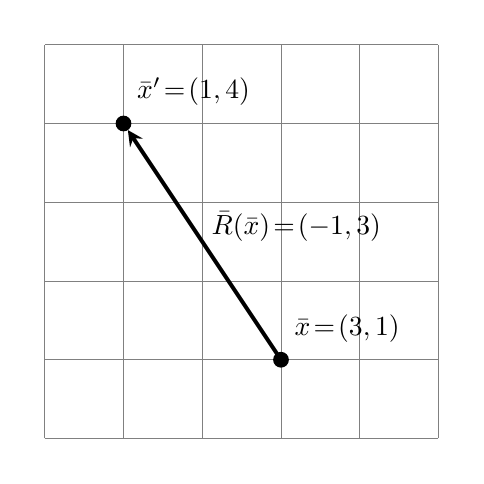
\begin{tikzpicture}
    \coordinate (bordernear) at (-0.1, -0.1);
    \coordinate (borderfar) at (5.1, 5.1);
    \coordinate (origin) at (0, 0);
    \coordinate (farcorner) at (5, 5);
    \coordinate (fixed) at (3,1);
    \coordinate (moved) at (1,4);
    \node at (bordernear){};
    \node at (borderfar){};
    \draw[gridlines] (origin) grid (farcorner);
    \node at (fixed)[gridnode]{};
    \node at (fixed)[nodelabel]{$\bar{x}\!=\!(3,1)$};
    \node at (moved)[gridnode]{};
    \node at (moved)[nodelabel]{$\bar{x}'\!=\!(1,4)$};
    \draw[mapvec] (fixed) to  node[mapveclabel]{$\bar{R}(\bar{x})\!=\!(-1,3)$} ($ (moved)!0.1cm!(fixed) $);


  \end{tikzpicture}
\end{document}
